%
% Main document
% ===========================================================================
% This is part of the document "Project documentation template".
% Authors: brd3
%

% Document informations
%---------------------------------------------------------------------------
\def \module		{Modul BTI7302 Projekt 2}	
\newcommand\mfTitle  {Modul BTI7302 Projekt 2}				% Module name
\def \title			{Disaggregation vom Stromverbrauch}			% Title
\def \version		{2.0}
\def \author		{Elisa Schnabel und Mathias Rudolf}
\newcommand\authoren{Elisa Schnabel, Mathias Rudolf}
\def \dozent		{Dr. Andreas Danuser}
\def \logo			{BFH_Logo_C_de_fr_en_100_4CU}	% choose the correct logo in
													% the folder Bilder/BFH_Logo
%---------------------------------------------------------------------------

%---------------------------------------------------------------------------
\documentclass[
	a4paper,				% paper format
	10pt,					% fontsize
%	twoside,				% double-sided
	oneside,				% one-sided
	openright,				% begin new chapter on right side
	notitlepage,			% use no standard title page
	parskip=half,			% set paragraph skip to half of a line
]{scrreprt}					% KOMA-script report
%---------------------------------------------------------------------------
\bibliographystyle{unsrt}
\raggedbottom
\KOMAoptions{cleardoublepage=plain}	% Add header and footer on blank pages


% Load Standard Packages:
%---------------------------------------------------------------------------
\usepackage[standard-baselineskips]{cmbright}

\usepackage[ngerman]{babel}		% german hyphenation
\usepackage[ansinew]{inputenc}  % Windows - load extended character set (ISO 8859-1)
\usepackage[T1]{fontenc}		% hyphenation of words with ä,ö and ü
\usepackage{textcomp}			% additional symbols
\usepackage{ae}					% better resolution of Type1-Fonts 
\usepackage{fancyhdr}			% simple manipulation of header and footer 
\usepackage{graphicx}			% integration of images
\usepackage{float}				% floating objects
\usepackage{caption}			% for captions of figures and tables
\usepackage{booktabs}			% package for nicer tables
\usepackage{tocvsec2}			% provides means of controlling the sectional numbering
\usepackage{rotating}			% rotating tables and other objects
\usepackage{pdflscape}			% change single pages landscape
\usepackage{tabularx}			% create nice tables
\usepackage{pdfpages}			% insert full pdf pages
\usepackage{nameref}			% reference by name, not by chapter number
\usepackage{dirtree}			% create directory trees
\usepackage{listings}			% include source code
\usepackage{epstopdf}			% convert eps graphics to pdf

%---------------------------------------------------------------------------

% Load Math Packages
%---------------------------------------------------------------------------
\usepackage{amsmath}			% various features to facilitate writing math formulas
\usepackage{amsthm}				% enhanced version of latex's newtheorem
\usepackage{amsfonts}			% set of miscellaneous TeX fonts that augment the standard CM
\usepackage{amssymb}			% mathematical special characters
\usepackage{exscale}			% mathematical size corresponds to textsize
%---------------------------------------------------------------------------

% Package to facilitate placement of boxes at absolute positions
%---------------------------------------------------------------------------
\usepackage[absolute]{textpos}
\setlength{\TPHorizModule}{1mm}
\setlength{\TPVertModule}{1mm}
%---------------------------------------------------------------------------					

% Definition of Colors
%---------------------------------------------------------------------------
\RequirePackage{color}							% Color (not xcolor!)
\definecolor{linkblue}{rgb}{0,0,0.8}			% Standard
\definecolor{darkblue}{rgb}{0,0.08,0.45}		% Dark blue
\definecolor{brickred}{cmyk}{0,0.89,0.94,0.28}	% Brickred
\definecolor{bfhred}{rgb}{0.776,0,0.066}		% Red
% specific colors
\definecolor{titlecolor}{rgb}{0,0,0}		% Color used for the title
%\definecolor{linkcolor}{rgb}{0,0,0.8}			% Blue for the web- and cd-version!
\definecolor{linkcolor}{rgb}{0,0,0}				% Black for the print-version!
\definecolor{code_bg}{gray}{0.8}				% Source Code Background
%---------------------------------------------------------------------------

% Hyperref Package (Create links in a pdf)
%---------------------------------------------------------------------------
\usepackage[
	pdftex,ngerman,bookmarks,plainpages=false,pdfpagelabels,
	backref = {false},					% No index backreference
	colorlinks = {true},				% Color links in a PDF
	hypertexnames = {true},				% no failures "same page(i)"
	bookmarksopen = {true},				% opens the bar on the left side
	bookmarksopenlevel = {0},			% depth of opened bookmarks
	pdftitle = {\title},				% PDF-property
	pdfauthor = {\author},			% PDF-property
	pdfsubject = {\module},			% PDF-property
	linkcolor = {linkcolor},			% Color of Links
	citecolor = {linkcolor},			% Color of Cite-Links
	urlcolor = {linkcolor},				% Color of URLs
]{hyperref}
%---------------------------------------------------------------------------

% Set up page dimension
%---------------------------------------------------------------------------
\usepackage{geometry}
\geometry{
	a4paper,
	left=28mm,
	right=15mm,
	top=30mm,
	headheight=20mm,
	headsep=10mm,
	textheight=232mm,
	footskip=15mm
}
%---------------------------------------------------------------------------

% Makeindex Package
%---------------------------------------------------------------------------
\usepackage{makeidx}			% To produce index
\makeindex						% Index-Initialisation
%---------------------------------------------------------------------------

% Glossary Package
%---------------------------------------------------------------------------
% the glossaries package uses makeindex
% if you use TeXnicCenter do the following steps:
%  - Goto "Ausgabeprofile definieren" (ctrl + F7)
%  - Select the profile "LaTeX => PDF"
%  - Add in register "Nachbearbeitung" a new "Postprozessoren" point named Glossar
%  - Select makeindex.exe in the field "Anwendung" ( ..\MiKTeX x.x\miktex\bin\makeindex.exe )
%  - Add this [ -s "%tm.ist" -t "%tm.glg" -o "%tm.gls" "%tm.glo" ] in the field "Argumente"
%
% for futher informations go to http://ewus.de/tipp-1029.html
%---------------------------------------------------------------------------
\usepackage[nonumberlist]{glossaries}
\makeglossaries

\newglossaryentry{BibTeX}{name={BibTeX},description={Programm zur Erstellung von Literaturangaben und -verzeichnissen in \TeX- oder \LaTeX-Dokumenten}}
\newglossaryentry{StwVrz}{name={Stichwortverzeichnis},description={Verzeichnis mit Stichworten aus dem Text}}



%---------------------------------------------------------------------------

% Listings Package
%---------------------------------------------------------------------------
\lstdefinestyle{CCode}{
	showspaces=false,
	showtabs=false,
	language={[ANSI]C},
	breaklines=true,
	basicstyle={\footnotesize \ttfamily},
	backgroundcolor=\color{code_bg},
	%frame=single,
	tab=\rightarrowfill,
	captionpos=b
}

\lstdefinestyle{CppCode}{
	showspaces=false,
	showtabs=false,
	language={[ISO]C++},
	breaklines=true,
	basicstyle={\footnotesize \ttfamily},
	backgroundcolor=\color{code_bg},
	%frame=single,
	tab=\rightarrowfill,
	captionpos=b
}

\lstdefinestyle{JavaCode}{
	showspaces=false,
	showtabs=false,
	language={Java},
	breaklines=true,
	basicstyle={\footnotesize \ttfamily},
	backgroundcolor=\color{code_bg},
	%frame=single,
	tab=\rightarrowfill,
	captionpos=b
}
%---------------------------------------------------------------------------

% Intro:
%---------------------------------------------------------------------------
\begin{document}				% Start Document
\settocdepth{section}			% Set depth of toc
\pagenumbering{roman}
%---------------------------------------------------------------------------

% Set up header and footer
%---------------------------------------------------------------------------
\fancyhf{}						% clean all fields
\fancypagestyle{plain}{			% new definition of plain style

% Use this for double-sided:
%	\fancyfoot[OL,ER]{\footnotesize				% footer left part -->	version
%		V\version \\
%		\author \\
%		\today
%	}
%	\fancyfoot[OR,EL]{\footnotesize \thepage}	% footer right part --> page number
%	\fancyhead[C]{\module}						% header right part --> module name
%	\fancyhead[OR,EL]{\footnotesize \leftmark}	% footer left part -->	chapter
%	\fancyhead[OL,ER]{							% header left part --> BFH logo
%		\begin{textblock}{0}[0,0](29,9)
%			\includegraphics[scale=1.0]{Bilder/\logo}
%		\end{textblock}
%	}

% Use this for one-sided:
	\fancyfoot[L]{\footnotesize					% footer left part -->	version
		V\version \\
		\author \\
		\today
	}
	\fancyfoot[R]{\footnotesize \thepage}		% footer right part --> page number
	\fancyhead[C]{\module}						% header right part --> module name
	\fancyhead[R]{\footnotesize \leftmark}		% footer left part -->	chapter
	\fancyhead[L]{								% header left part --> BFH logo
		\begin{textblock}{0}[0,0](29,9)
			\includegraphics[scale=1.0]{Bilder/BFH_Logo/\logo}
		\end{textblock}
	}
}

\renewcommand{\chaptermark}[1]{\markboth{\thechapter.  #1}{}}
\renewcommand{\headrulewidth}{0pt}				% no header stripline
\renewcommand{\footrulewidth}{0pt}				% no bottom stripline

\pagestyle{plain}
%---------------------------------------------------------------------------


% Title Page and Abstract
%---------------------------------------------------------------------------

% Project documentation template
% ===========================================================================
% This is part of the document "Project documentation template".
% Authors: brd3
%

\begin{titlepage}


% BFH-Logo absolute placed at (29,10) on A4
% Actually not a realy satisfactory solution but working.
%---------------------------------------------------------------------------
\begin{textblock}{0}[0,0](29,10)
	\includegraphics[scale=1.0]{Bilder/BFH_Logo/\logo}
\end{textblock}

% Titel / Untertitel / Autor:
%---------------------------------------------------------------------------


\vspace*{2cm}

\fontsize{18pt}{20pt}\selectfont
\centering
\mfTitle \\
\fontsize{12pt}{15pt}\selectfont\vspace{0.5em}


\vspace{2cm}

\fontsize{30pt}{32pt}\selectfont 
\centering \textcolor{titlecolor}{\textbf{\title}} \\

\vspace{7cm}
\fontsize{12pt}{15pt}\selectfont
\begin{tabbing}
xxxxxxxxxxxxxxxx\=xxxxxxxxxxxxxxxxxxxxxxxx	\kill
Autoren:			\> \authoren					\\
Datum:			\> \today					\\
Version:		\> \version					\\
Dozent:			\> Dr. Andreas Danuser				\\
\end{tabbing}


\vspace{1cm}
\fontsize{12pt}{15pt}\selectfont
\begin{flushleft}
Hier kommt ein Abstrakt....


\end{flushleft}

\end{titlepage}

%
% ===========================================================================
% EOF
%

\cleardoubleemptypage
\setcounter{page}{1}

%---------------------------------------------------------------------------

% Table of contents and listings
%---------------------------------------------------------------------------
\tableofcontents
\listoffigures
\cleardoublepage
%---------------------------------------------------------------------------

\pagenumbering{arabic}
\settocdepth{subsection}		% Set depth of toc

% Main part - Part I
%---------------------------------------------------------------------------

\label{part:teil1}
\onecolumn
\chapter{Einleitung}
\label{chap:teil1_einleitung}

Ein intelligentes Z�hlersystem, das einzelne Verbraucher aus dem Gesamtstromverbrauch erkennen kann -- dieser anspruchsvollen Aufgabe widmet sich diese Projekt 2 Arbeit. Der zugrunde liegende Gedanke des Projektes ist es, dass jeder einzelne Verbraucher Strom und Spannung in unterschiedlicher Art und Weise beeinflusst und damit eine Art "` Signatur "'  im Stromnetz hinterl�sst. Diese Signatur wird als aggregierter Gesamtstromverbrauch von einem Smart Meter (EM340) erfasst. Mittels Neuronalen Netzen, eventbasierten Algorithmen oder schon mittels einfacher Kombinatorik k�nnen Muster im Gesamtstromverbrauch erkannt und einzelnen Verbrauchern zugeordnet werden. Im Gegensatz zum Submetering Verfahren, welches mit mehreren Z�hlern arbeitet, identifiziert dieses System mit einem einzigen Z�hler die aktiven Verbraucher, welche an das Stromnetz angeschlossen sind. Damit werden nicht nur Kosten f�r die Messhardware sowie Installation und Wartungsaufw�nde, sondern auch Stromkosten gespart. Denn die eigenen Stromkosten senken kann nur derjenige wirklich effektiv, der seinen Stromverbrauch kennt und genau weiss, bei welchen Verbrauchern er bzw. sie mit dem Sparen ansetzen kann. Somit erm�glicht dieses System auch die verursachergerechte Aufteilung der anfallenden Energiekosten. Das bedeutet, dass sich jedem Verbraucher exakt die Energiekosten zuordnen lassen, die f�r dessen Betrieb angefallen sind. Dies mag sich f�r Privathaushalte m�glicherweise nicht interessant anh�ren, in der Wirtschaft dagegen umso mehr.   

\chapter{Motivation / Ziele}
\label{chap:teil1_motziel}
Die Nachfrage nach Energie w�chst weltweit rasant, und die Nachfrage nach elektrischer Energie w�chst noch schneller [1]. Die Nachfrage nach elektrischer Energie wird sich bis zum Jahre 2050 voraussichtlich verdoppeln [2]. Um diese Energieprobleme zu l�sen, ist es notwendig, Elektrizit�t wirtschaftlch und intelligent zu nutzen. Ein Ansatz zur Steigerung der Effizienz des Stromverbrauchs besteht darin, positive Verhaltens�nderungen bei den Verbrauchern anzuregen. Dies kann durch Analysen des Energieverbrauchs erreicht werden. Non-Intrusive Load Monitoring (NILM) ist eine geeignete Methode dazu. NILM ist ein Prozess zur Analyse von �nderungen der Spannung und des Stroms, die in ein Haus gehen, und leitet daraus ab, welche Verbraucher im Haus mit ihrem individuellen Energieverbrauch verwendet werden.

Das prim�re Ziel dieser Projekt 2 Arbeit ist es erstmal, sich mit dem ganzen Thema rund um NILM vertraut zu machen. Dazu geh�rt auch sich die elektrotechnischen Grundlagen zu erarbeiten, welche als Basis zur Signaturerstellung der Verbraucher dienen. Denn um einen Energieverbrauch basierend auf NILM zu disaggregieren, muss man die Funktionsweise der Verbraucher verstehen.
Die Disaggregation soll in einem ersten Schritt mit einfacher Kombinatorik implementiert werden. In einem n�chsten Schritt wird ein eventbasierter Ansatz angewendet. Als Zusatz soll dann das Disaggregationsverfahren noch im Hinblick auf Machine Learning und Neuronale Netze untersucht werden.

% Eintr�ge im Verzeichnis erscheinen lassen ohne hier eine Referenz einzuf�gen
\nocite{raichle:bibtex_programmierung}
\nocite{MiKTeX}
\nocite{KOMA}
\nocite{TeXnicCenter}












% Main part - Part 1
%---------------------------------------------------------------------------

\label{part:teil1}
\onecolumn
\chapter{�bersicht Gesamtsystem}
\label{sec:teil1_uebersicht}

Das System besteht aus einem Smart Meter (EM340) und einem Gateway, auf welchem die Software zur Verbrauchsanalyse installiert ist. Die Ger�te sind alle an der Phase L1 des Energiez�hlers angeschlossen. Prinzipiell ist der hier verwendete Energiez�hler  zwar so konzipiert, dass er auf drei verschiedenen Phasen Messungen durchf�hren k�nnte, in diesem Projekt wurde aber auschliesslich die Phase L1 genutzt.

TODO: Grafik SIOT erg�nzen 

\begin{figure}[H]
	\centering
	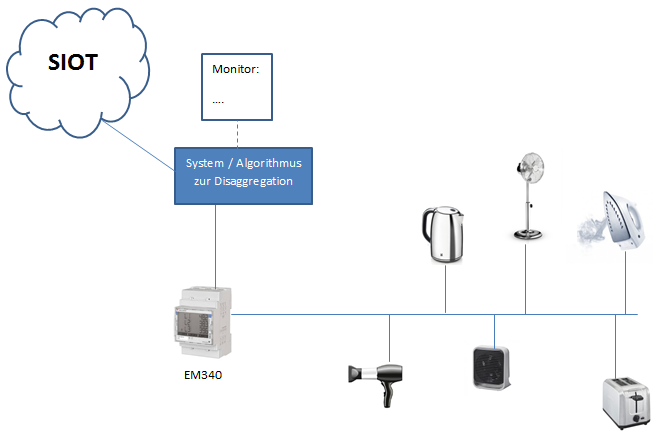
\includegraphics[width=1.0\textwidth]{Bilder/uebersicht.png} %70% der Textbreite
	\caption{�bersicht Gesamtsystem}
	\label{fig:teil1_pestle}
\end{figure}

Als Gateway dient hier ein Raspberry Pi, auf welchem das in Python geschriebene Programm l�uft,mit welchem die Daten aus dem Z�hler gelesen, verarbeitet und an das SIOT gesendet werden. Der Energiez�hler stellt verschiedene Register bereit, aus welchen jeweils pro Phase der Stromverbrauch I [A], die Spannung U [V], die Wirk P [W]-, Schein S [VA]- und Blindleistung Q [var] herausgelesen werden k�nnen. Diese Werte bilden die Grundlage zur Signaturerstellung der einzelnen Verbraucher.

\chapter{Erstellen von Signaturen der Verbraucher}
\label{sec:teil1_uebersicht}
Aufgrund der physikalischen Gegebenheiten beeinflusst jedes Haushaltsger�t Strom und Spannung auf unterschiedliche weise. Genauer gesagt unterscheidet man zwischen ohmschen-, kapazitiven- und induktiven Verbrauchern. Ohmsche Verbraucher bestehen aus einem oder mehreren Widerst�nden, d.h. elektrischen Komponenten, die im wesentlichen Hitze oder Licht erzeugen. Beispiele daf�r sind der Ofen, Gl�hbirnen oder B�geleisen. Beim rein ?ohmschen? Verbraucher (dem ohne induktiven oder kapazitiven Anteil) sind Spannung und Strom stets ?in Phase?, d.h. es gibt keine Phasenverschiebung und somit keinen Blindleistungsanteil, was gleichzeitig auch bedeutet, dass die Wirkleistung gleich der Scheinleistung entspricht. Induktive Verbraucher sind im wesentlichen elektromagnetische Verbraucher, d.h. elektrische Komponenten, die Elektromagnetismus erzeugen. Diese Ger�te ben�tigen beim Anlauf unter Umst�nden ein vielfaches an Anlaufstrom. Beispiele daf�r sind Pumpen oder auch Ventilatoren. Bei rein induktiven Komponenten eilt die Spannung dem Strom voraus, wodurch sich eine Phasenverschiebung von 90 Grad ergibt. D.h. hier gibt es einen Blindleistungsanteil und somit ist die Wirkleistung ungleich der Scheinleistung. Kapazitive Verbraucher verhalten sich �hnlich wie induktive Verbraucher, mit dem unterschied, dass hier keine Magnetfelder aufgebaut werden, sondern elektrische Felder. Bei kapazitiven Lasten eilt der Strom der Spannung voraus, wobei auch hier wieder eine Phasenverschiebung von 90 Grad entsteht. D.h. also, dass auch kapazitive Lasten einen Blindleistungsanteil besitzen und die Wirkleistung nicht der Scheinleistung entspricht. Allerdings sind rein ohmsche, kapazitive und induktive Verbraucher eher selten und Misch-Verbraucher die Regel. D.h. also dass jeder Verbraucher in unterschiedlicher Weise Wirk-, Blin-, und Scheinleistung beeinflusst. Somit k�nnten zwei Verbraucher mit gleicher Wirkleistung trotzdem unterschieden werden aufgrund unterschiedlicher Blindleistungsanteilen. 

TODO: Grafiken induktiv, kapazitiv, ohmsche aus Wiki

Um f�r jedes Haushaltsger�t eine Signatur erstellen zu k�nnen, werden die Ger�te zu Beginn jeweils einzeln an das Smartmeter angeschlossen und die jeweiligen Register �ber einen Zeitraum von 30 Sekunden ausgelesen. Die so gewonnenen Daten werden anschliessend in einer Datenbank abgespeichert und einem Ger�t eindeutig zugewiesen. Diese Signatur wird dann schlussendlich verwendet um den Gesamtstromverbrauch auf die einzelnen Verbraucher aufschl�sseln zu k�nnen. F�r diess Projekt 2 Arbeit kamen folgende Haushaltsger�te zum Einsatz: Haarf�hn, Heizl�fter, Ventilator, B�geleisen, Toaster, Wasserkocher und Stabmixer. Die erstellten Signaturen werden auf folgenden Abbildungen illustriert. 

TODO: 3 Beispielgrafiken (Wasserkocher und tbd)
\chapter{Einleitung}
\label{chap:teil1_einleitung}\chapter{Einleitung}
\label{chap:teil1_einleitung}

\begin{figure}[H]
	\centering
	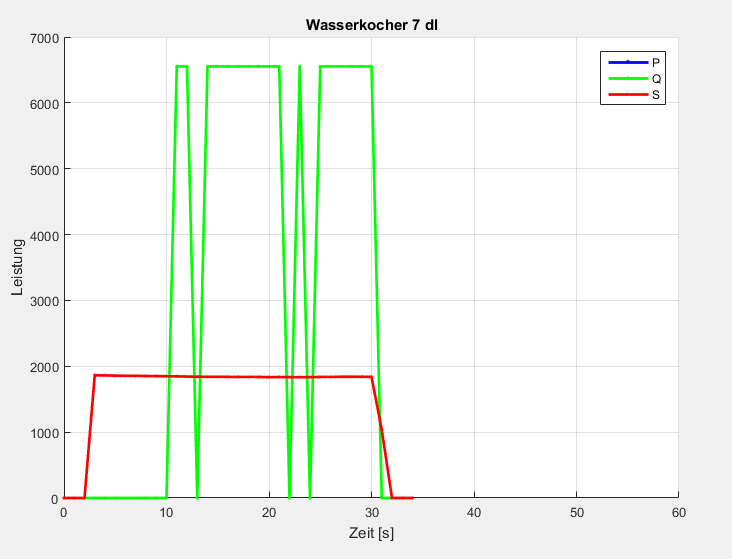
\includegraphics[width=0.5\textwidth]{Bilder/wasserkocher.png} %70% der Textbreite
	\caption{�bersicht Gesamtsystem}
	\label{fig:teil1_pestle}
\end{figure}

\chapter{Disaggregation: Ansatz mittels Kombinatorik}
\label{sec:teil1_kombinatorik}
-Algorthmus beschreiben (Inputs, Berechnungen) ev. Codebeispiele (eher mathematisch beschreiben)


\chapter{Ergebnisse}
\label{sec:teil1_kombinatorik}
-Ergebnisse (genauigkeit was wurde erkannt, was gibt es f�r Probleme mit dem Ansatz?
-Tabellarische Auflistung der erkannten bzw. nicht erkannten Ger�ten

\chapter{Ansatz Machine Learning}
\label{sec:teil1_kombinatorik}
-Wie w�rde dieser Ansatz funktionieren? beschreiben. NN und ML?

\chapter{Schlusswort}
\label{sec:teil1_kombinatorik}

Fazit, Schwierigkeiten, Ausblick Thesis
% Eintr�ge im Verzeichnis erscheinen lassen ohne hier eine Referenz einzuf�gen
\nocite{kopka:band1}
\nocite{raichle:bibtex_programmierung}
\nocite{MiKTeX}
\nocite{KOMA}
\nocite{TeXnicCenter}
\nocite{Marti06}
\nocite{Erbsland08}
\nocite{juergens:einfuehrung}
\nocite{juergens:fortgeschritten}











%---------------------------------------------------------------------------

%---------------------------------------------------------------------------
\end{document}
